\documentclass{beamer}
% September 2014 
% Author: Dr Rachid Hourizi and Dr. Michael Wright 
% Department of Computer Science, University of Bath
\usepackage{listings}
\usetheme{Boadilla} 
\usepackage{fixltx2e}
\usepackage{hyperref}
\lstset{language=Java}

\begin{document}

\AtBeginSection[]{
  \begin{frame}
  \vfill
  \centering
  \begin{beamercolorbox}[sep=8pt,center,shadow=true,rounded=true]{title}
    \usebeamerfont{title}\insertsectionhead\par%
  \end{beamercolorbox}
  \vfill
  \end{frame}
}

\title{CM 10227: Lecture 8b}
\author{Dr Rachid Hourizi and Dr. Michael Wright}
\date{\today}
\frame{\titlepage}

\section{Java In/Out: In}
\begin{frame}

\begin{itemize}
\item To this point,  we have looked at ways in which 
\begin{itemize}
\item Information can be passed to a program as part of an instruction to run (command line parameters) and
\item Objects can pass information to (and receive information from) other Objects 
\end{itemize}
\item We have not, however, looked at the ways in which the user can interact with our code whilst it is running
\item The following slides will introduce the basics of passing Java input to a running program from a command line or console 
\item (Note that receiving user input via a graphical user interface is handled separately and will be covered in Semester 2)
\end{itemize}

\end{frame}

\begin{frame}
\begin{itemize}
\item A good starting point for discussion of Input and Output is to consider the idea of a stream
\item In contrast to the Arrays we saw earlier in the course, streams are (at least potentially) unlimited sequence of data 
\item As far as a running Java program knows, the data coming from a user's keyboard or a file

\begin{itemize}
\item Is not of fixed length
\item And could (in theory at least) be infinite
\end{itemize}
\item Similarly the amount of data that could (again in theory) be sent to a screen, printer or output file could also
be infinite
\end{itemize}
\end{frame}

\begin{frame}
\begin{itemize}
\item With that in mind, Java provides us with both input and output streams that we can use to
\begin{itemize}
\item Read from a stream of input and
\item Write a stream of output to a designated destination (the screen, a file etc)
\end{itemize}
\item Collectively, those input (I) and output (O) streams are described as IO streams
\item This week, we will take a first look at input streams
\end{itemize}

\end{frame}
\begin{frame}

\begin{itemize}
\item As usual with Java classes, we do not need to know how IO streams provide the functionality that they do 
\item We don't, for example, need to know how they

\begin{itemize}
\item capture of data from a source (e.g. the keyboard)
\item transmit data to a final destination (e.g. the screen)
\end{itemize}
\item We simply have to know and be able to use the interface that those classes provide in order to

\begin{itemize}
\item Read data into a Java program and
\item Write data from it
\end{itemize}
\end{itemize}

\end{frame}

\begin{frame}

\begin{itemize}
\item From http://tutorials.jenkov.com/java-io/streams.html:

\begin{itemize}
\item Java IO streams are flows of data you can either read from, or write to.
\item IO Streams are typically connected to a data source, or data destination, like a file,
network connection etc.
\item A stream has no concept of an index of the read or written data, like an array does. 
\item Nor can you typically move forth and back in a stream, like you can in an array
\item A stream is just a continuous flow of data.
\end{itemize}
\end{itemize}
\end{frame}

\begin{frame}
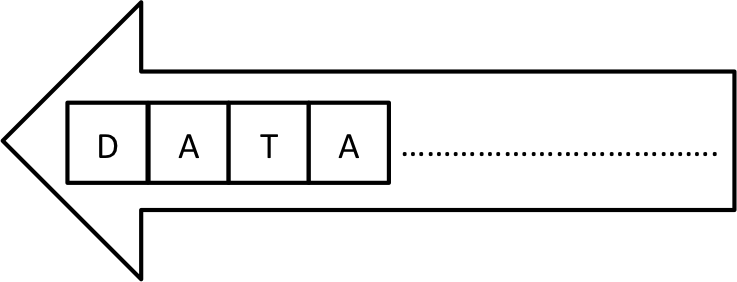
\includegraphics[scale=0.5]{Stream1.png}
\end{frame}

\begin{frame}
\begin{itemize}
\item We have already introduced three of the streams that are available to Java at runtime

\begin{itemize}
\item Standard in
\item Standard out
\item Standard error
\end{itemize}
\item Java calls these three streams

\begin{itemize}
\item System.in
\item System.out
\item System.err
\end{itemize}
\end{itemize}

\end{frame}

\begin{frame}

\begin{itemize}
\item The 3 streams System.in, System.out, and System.err are common sources or destinations of data
\item These 3 streams are initialized by .. Java … when (it) starts up, so you don't have to instantiate them yourself (although you can exchange them at runtime).
\item Most commonly used is probably System.out for writing output to the console from console programs
\end{itemize}

\end{frame}\begin{frame}

\begin{itemize}
\item System.out

\begin{itemize}
\item System.out is a PrintStream. 
\item System.out normally outputs the data you write to it to the console. 
\item This is often used from console-only programs like command line tools. 
\item This is also often used to print debug statements of from a program (though it may arguably not be the best way to
get debug info out of a program).
\end{itemize}
\end{itemize}

\end{frame}\begin{frame}

\begin{itemize}
\item System.err

\begin{itemize}
\item System.err is also a PrintStream. 
\item System.err works like System.out except it is normally only used to output error texts. 
\item System.err often prints to the same location as System.out (the screen)
\item Some programs (like Eclipse) will show the output to System.err in red text, to make it more obvious that it is
error text.
\end{itemize}
\end{itemize}

\end{frame}

\begin{frame}[fragile]
\small
\begin{block}{}
\begin{lstlisting}
public class ExampleCode {
	public static void main(String[] args) {
        
        //printing to System.out
        System.out.println("Desired Output");
        
        //printing to System.err
        System.err.println("Informtion about an error");

    }
}
\end{lstlisting}
\end{block}

\begin{block}{}
\begin{lstlisting}
both outputs print to the screen:

rachidhourizi$ java Examplecode
Desired Output
Informtion about an error that has occurred

\end{lstlisting}
\end{block}

\end{frame}

\begin{frame}

\begin{itemize}
\item System.in

\begin{itemize}
\item System.in is an InputStream which is typically connected to keyboard input. 
\item In applications with GUI the input to the application is given via the GUI. This is a separate input mechanism
from Java IO.
\end{itemize}
\end{itemize}

\end{frame}\begin{frame}

\begin{itemize}
\item A group of Java classes take IO streams (e.g. Standard in, Standard our and Standard
error) as input and return that data in more manageable chunks
\end{itemize}
\end{frame}

\begin{frame}[fragile]
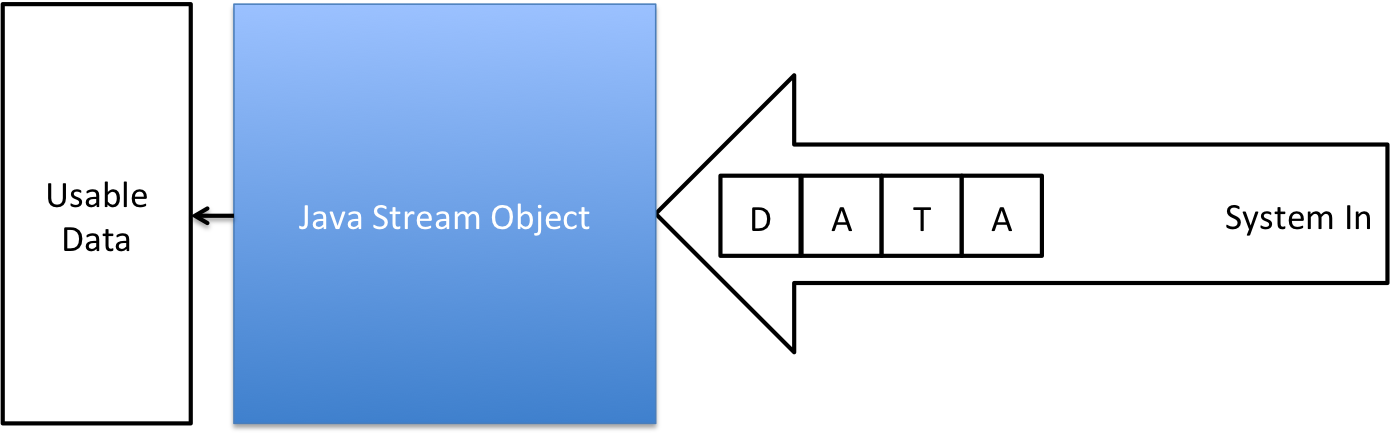
\includegraphics[scale=0.5]{Stream2.png}
\end{frame}

\begin{frame}
Different Classes return data in different forms:
\begin{itemize}
\item Some IO classes allow us to access data byte by byte (e.g. InputStream)
\item Others give each line of data as a String (e.g. BufferedReader)
\item And others help us to interpret (``parse'') the incoming data (e.g. Scanner)
\end{itemize}
\end{frame}


\begin{frame}
\begin{itemize}
\item We will look at the family of IO classes in more detail in the coming weeks
\item At this point, however, we simply need to be able to
\begin{itemize}
\item read data from an input stream
\item and pass that data to the rest of our code (e.g. SRPN)
\end{itemize}
\end{itemize}
\end{frame}

\begin{frame}
\begin{itemize}
\item Passing data from System.in to a Bufferedreader requires us to take two steps:
\begin{itemize}
\item First we have to create an instance of the InputStreamReader class (an InputStreamReader Object) and attach it to System.in
\item this can be done by calling the InputStreamReader constructor and passing it System.in as a parameter:

\begin{itemize}
\item new InputStreamReader(System.in)
\end{itemize}


\item the InputStreamReader Object will take the stream of information coming from Standard.in and passes it to BufferedReader one char at a time

\end{itemize}
\end{itemize}

\end{frame}

\begin{frame}
\begin{itemize}
\item Second, we have to call the BufferedReader constructor and pass it the InputStreamReader Object as a parameter
\begin{itemize}
\tiny
\item BufferedReader br = new BufferedReader(new InputStreamReader(System.in));
\end{itemize}
\item as a reult, we have a chain of Java IO objects: 
\item the InputStreamReader Object will take the stream of information coming from Standard.in and passes it to BufferedReader one char at a time
\item BufferedReader will take that stream of chars and buffer them (store multiple chars ready for processing), presenting us with a String containing  all the chars up to the point that the user presses enter on the keyboard
\end{itemize}
\end{frame}

\begin{frame}
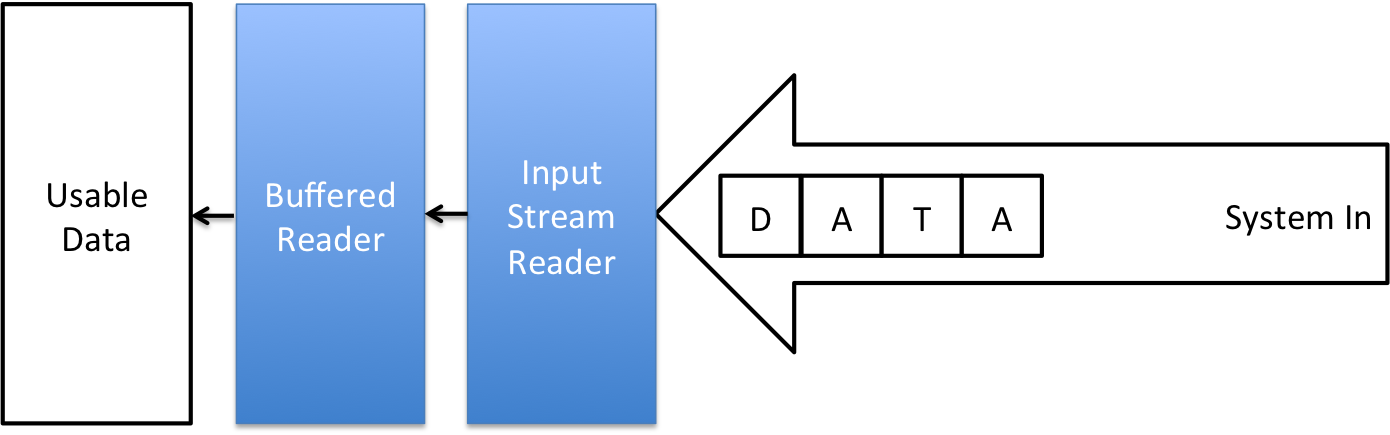
\includegraphics[scale=0.5]{Stream3.png}
\end{frame}

\scriptsize
\begin{frame}[fragile]
\begin{block}{}
\begin{lstlisting}
import java.io.BufferedReader;
import java.io.InputStreamReader;

public class BufferedReaderX {
   public static void main(String[] args) throws Exception {

	  //create String to hold output from BufferedReader
	  String s;
      
      // create InputStreamReader Object
      // attach it to the stream of data coming from System.in
      // and use it to create a new BufferedReader Object
      BufferedReader br = 
              new BufferedReader(new InputStreamReader(System.in));
      
      //ask user to make a first input 
      System.out.println("Please enter something");
      
      //print out the user's last input and ask for further input
      while ((s=br.readLine()) != null) {
            System.out.println("You entered " + s 
                 + " Please enter something else");
      }       
   }
}
\end{lstlisting}
\end{block}
\end{frame}

\begin{frame}
\begin{itemize}
\item At this point, you know how to read information in from System.in (i.e. from the user) one String at a time
\item The example on the previous slide simply prints each String s to screen
\item But for SRPN, you will need to look more closely at each incoming String
\item Identify the different pieces of infomration within it 
\item i.e. operators and operands
\item store those operators and operands somewhere 
\item ... and then perform the mathematical operations that they describe
\end{itemize}
\end{frame}

\begin{frame}
\begin{itemize}
\item The following slides will give you some assistance as you think about how to write SRPN
\item They will not, however, provide you with solutions that you can use ``As-is'' in your coursework
\item If you cannot work out how to construct the SRPN using these building blocks, ask in the labs, post to programming1 etc.
\end{itemize}
\end{frame}


\begin{frame}
\begin{itemize}
\item It is tempting to start by passing the information from System.in  to a ``Scanner''
\item Scanner is an extremely helpful pre-written Class which allows you to extract the information in the String provided by System.in (or a BufferedReader) as one or more Integers, Floats etc.
\item In order to use that class, you would set up a ``chain'' of Java IO Objects similar to the ones on the diagram above
\item System.in -- Scanner -- Your Code
\item or
\item System.in -- BufferedReader -- Scanner -- Your Code
\end{itemize}
\end{frame}

\begin{frame}[fragile]
\begin{block}{}
\begin{lstlisting}
import java.util.Scanner;  
class ScannerTest{  
 public static void main(String args[]){  
   Scanner sc=new Scanner(System.in);  
   System.out.println("Enter your name"); 
   String name=sc.next();  
   System.out.println("Enter an Integer");  
   int myNumber=sc.nextInt();  
   System.out.println("Your name is: "+name +"Your number is: "+myNumber);  
   sc.close();  
 }  
}  
\end{lstlisting}
\end{block}
\begin{block}{}
\begin{lstlisting}
 Enter your name
 Rachid
 Enter an integer
 100
Your name is:Rachid Your number is:100
\end{lstlisting}
\end{block}
\begin{itemize}
\item Note the use of an import statement (somewhat similar to the include statements we saw in C)
\item note also the use of the .next() method to pull out the next block of text from System.in
\item note also the use of the .nextint() method to pull out the next integer from System.in
\end{itemize}
\end{frame}

\begin{frame}
\begin{itemize}
\item You should note, however, that Scanner requires a recognisable separator (``delimiter'') to exist between the chunks of information that it processes
\item By default, Scanner expects white space (i.e. a space or a tab etc.) to be used to separate on piece of information from another
\item though you can instruct a Scanner Object to look for other delimiters (e.g. commas)
\item \textbf{This is a problem if the chunks of information (``tokens'') being fed to your program are not separted by white space}
\item e.g. Scanner would not interpret ``4+3'' (no spaces) as an int followed  by an operator followed by another int
\item it would see only a single String
\end{itemize}
\end{frame}

\begin{frame}
\begin{itemize}
\item you can get some way into the SRPN exercise using a Scanner to interpret input
\item but will need to adopt an alternative approach if you want to pass all of our automated tests
\bigskip
\item You might want to do exactly that (Start with a Scanner and then change the way your code reads input) as part of an iterative programming approach
\end{itemize}
\end{frame}

\begin{frame}
\begin{itemize}
\item An alternative approach is to read in each line of input as a String (using BufferedReader - see the example in a earlier slide)
\item and then to analyse that String for yourself
\end{itemize}
\end{frame}

\begin{frame}[fragile]
\begin{itemize}
\item In order to do that, you may want to take advantage of methods defined by the String class e.g.:
\begin{itemize}
\small
\item charAt(int); //returns the character at the given index (position) in a String
\item getNumericValue(char) // returns the value of the given char interpreted as an int
\end{itemize}
\end{itemize}
\begin{block}{}
\begin{lstlisting}
String element = "el5";
int x = Character.getNumericValue(element.charAt(2));
System.out.println("x=" + x);
\end{lstlisting}
\end{block}
\begin{block}{}
\begin{lstlisting}
x=5
\end{lstlisting}
\end{block}
\end{frame}


\begin{frame}[fragile]
\begin{itemize}
\item For (large) numbers represented by mulitple characters, you may want to extract a part of the input string (``substring'') before interpreting the value
\begin{block}{}
\begin{lstlisting}
import java.io.*;
public class Test {

   public static void main(String args[]) {
      String s1 = new String("HelloWorld");
      String s2 = new String(s1.substring(1,4));

      System.out.println(s2);
   }
}
\end{lstlisting}
\end{block}
\begin{block}{}
\begin{lstlisting}
ello
\end{lstlisting}
\end{block}
\end{itemize}
\end{frame}


\begin{frame}
\begin{itemize}
\item One final step is to convert the String (or substring) provided by BufferedReader and convert it to an int (for use in the mathematical calculations performed by SRPN)
\item this can be with the Integer.parseInt() method
\begin{itemize}
\item int foo = Integer.parseInt("1234");
\end{itemize}
\item This code snippet would leave us with variable foo holding the value 1234
\end{itemize}
\end{frame}


\begin{frame}
\begin{itemize}
\item You may want to check that you have a String that can be converted to an Int before using ParseInt()
\item this can be done with the Character.isDigit(char) method e.g.
\begin{itemize}
\item boolean check = Character.isDigit(char); 
\end{itemize}
\item This method takes in a char
\item ...returns true if that Char can be interpreted as an int
\item ...and returns false if the input is not a char that can be interpreted as an int
\item Note that you will have to check each char individually (using a loop and charAt()) to see whether the String that you want to check contains a multi-digit integer
\end{itemize}
\end{frame}

\begin{frame}
\begin{itemize}
\item At this point, it is important to know to know that it is \textbf{not} possible to describe all elements in a Java program using Class and Object diagrams:
\bigskip 
\item In fact, Java defines two very different categories of data type:
\item primitive types

\begin{itemize}
\item int, char, boolean etc.
\end{itemize}
\item object types

\begin{itemize}
\item ArrayList, LinkedList, TicketMachine
\end{itemize}
\end{itemize}

\end{frame}

\begin{frame}

\begin{itemize}

\item Object types originate from classes.
\begin{itemize}
\item Some of which are predefined and 
\item Some of which we can write ourselves
\end{itemize}
\end{itemize}

\begin{itemize}
\item The primitive types are non-object types.
\begin{itemize}
\item Have no constructors, accessors, mutators
\end{itemize}
\item All primitive types are predefined by Java.
\bigskip
\item An aside: This means that Java is not a completely object oriented language
\end{itemize}

\end{frame}
\begin{frame}[fragile]
\begin{block}{}
\begin{lstlisting}
//asignement of a primitive to a variable 
//without a call to a constructor
int a = 6;

//asignment of an Object to a variable 
//using a constructor call
TicketMachine t = new TicketMachine(500);

\end{lstlisting}
\end{block}
\end{frame}


\begin{frame}

\begin{itemize}
\item There are eight primitive data types supported by Java

\begin{itemize}
\item byte (8-bit singed integer)
\item short (16-bit signed integer)
\item int (32-bit signed integer)
\item long (62-bit signed integer)
\item float (32-bit floating point number)
\item double (64-bit floating point number)
\item boolean (single bit true/false)
\item char (16-bit Unicode character)
\end{itemize}
\end{itemize}

\end{frame}

\begin{frame}[fragile]

\begin{itemize}
\item There are situations in which Java requires the use of an Object
\item With this in mind, Java provides ``wrapper classes'';

\begin{itemize}
\item Classes which, when instantiated \textbf{do} provide objects 
\item And hold the same values as the primitives used to create them
\end{itemize}
\end{itemize}

\end{frame}


\begin{frame}

\begin{itemize}
\item Wrapper classes can be thought of as a way to make an Object from a primitive
\item Wrapper classes mostly have the same name as the underlying primitive
\item But the first letter is capitalized
\begin{itemize}
\item The wrapper class for byte is therefore Byte
\item boolean is Boolean 
\item and so on 
\end{itemize}
\item Two notable exceptions are
\begin{itemize}
\item int: The wrapper class for int is Integer
\item char: The wrapper class for char is Character
\end{itemize}
\end{itemize}
\end{frame}

\begin{frame}
\begin{definition}[Boxing]
Converting a primitive to a (wrapper) object \newline e.g. an int to Integer\newline is called boxing.
Converting an Integer to int is called unboxing
\end{definition}
\begin{definition}[Unboxing]
Converting a (wrapper) object to a primitive\newline e.g. an Integer to an int\newline is called boxing.
Converting an Integer to int is called unboxing
\end{definition}
\end{frame}



\begin{frame}[fragile]

\begin{itemize}
\item Wrapper classes have constructors, just as you would expect of any other class
\end{itemize}

\begin{block}{}
\begin{lstlisting}
//primitive
int a=7;

//constructing an Integer wrapper object using that primitive
Integer b = new Integer(a);

\end{lstlisting}
\end{block}

\end{frame}

\begin{frame}[fragile]

\begin{itemize}
\item Wrapper classes also provide accessors
\item So using them as you would use primitives is poor practice
\item But using them with an accessor method is acceptable
\end{itemize}

\begin{block}{}
\begin{lstlisting}
int a = 7;
Integer b = new Integer(5);

//intValue returns the value held 
//in the Integer object as an int
a = a + b.intValue() 

\end{lstlisting}
\end{block}
\begin{itemize}
\item Note: these accessors return primitives
\begin{itemize}
\item e.g. in the example above, the returned value is an int (primitive)
\end{itemize}
\end{itemize}
\end{frame}

\begin{frame}[fragile]
\begin{itemize}
\item Wrapper classes are immutable, so they dont provide mutators
\item Note however that Java does handle \textbf{some} boxing and unboxing (conversion to and from primitives) automatically so it will, in some circumstances look as a program is using the value contained within a wrapper object without an accessor
\end{itemize}

\begin{block}{}
\begin{lstlisting}
//example of automatic unboxing
Integer a=3;
Integer b=3;
a+=b;
System.out.println(a);

\end{lstlisting}
\end{block}
\end{frame}

\begin{frame}[fragile]
\begin{itemize}
\item Usefully, the wrapper classes also include accessor methods which return the value held as primitives of another type
\item E.g. the Integer wrapper class provides the floatValue() method to return the underlying int as a float primitive:
\end{itemize}

\begin{block}{}
\begin{lstlisting}
float a = 7.0f;
Integer b = new Integer(5);

//floatValue() method returns the value held 
//in the Integer object as a float
a = a + b.floatValue();

//print result
System.out.println(a);
\end{lstlisting}
\end{block}

\begin{block}{}
\begin{lstlisting}
Output is: 12.0

\end{lstlisting}
\end{block}
\end{frame}

\begin{frame}[fragile]
\begin{itemize}
\item The wrapper classes also include \textbf{static} methods which return the value represented by a String as a boxed object
\item E.g. the Integer wrapper class provides a method to return the value represented by a String as an int primitive
\end{itemize}

\begin{block}{}
\begin{lstlisting}
String s ="10";
int a;

a= Integer.parseInt(s); 
a=a+1;
System.out.println(""+a);

\end{lstlisting}
\end{block}

\begin{block}{}
\begin{lstlisting}
Output is: 11

\end{lstlisting}
\end{block}
\begin{itemize}
\item Static methods are provided by a class not by an object of that class
\item This means that we dont need to create an instance of Integer (an Integer object) to use parseInt()
\item We will return to the idea of static methods later in the course
\end{itemize}
\end{frame}

\end{document}